\documentclass[xcolor={svgnames}]{beamer}
\usetheme[progressbar=frametitle]{metropolis}

\usepackage{graphicx}
\usepackage{courier}
\usepackage{listings}

\usepackage[autostyle]{csquotes}
\usepackage[
    backend=biber,
    style=authoryear-icomp,
    sortlocale=de_DE,
    natbib=true,
    url=false, 
    doi=false,
    eprint=false
]{biblatex}
\addbibresource{biblio.bib}

\usepackage[svgnames]{xcolor}
\xdefinecolor{darkgreen}{named}{DarkGreen}

\lstdefinelanguage{lustre}{%
   columns=fullflexible,%
   basicstyle=\tt\footnotesize,
   % keywordstyle=\bfseries,
   commentstyle=\slshape,%
   keywords={%
     node,var,let,tel,returns,
     when,merge
   },%
   keywordstyle={\color{darkgreen}\sffamily},%
   morekeywords=[2]{%
     int, real, bool,
   },%
   keywordstyle=[2]{\color{blue}\ttfamily},%
   classoffset=2,%
   morekeywords=[3]{%
     storage, parameter, code %
   },%
   morekeywords=[3]{
     True,False
   },
   keywordstyle=[3]{\color{purple}},%
   sensitive,%
   morestring=[d]",%"
}[keywords,comments,strings]%

\lstMakeShortInline[language=albert]?

\lstset{language=lustre}

\title{Un compilateur pour le langage Minilucy}
\author{Basile Pesin}

\begin{document}

\maketitle

\section{Organisation du projet}

\begin{frame}{Choix techniques}
  \begin{itemize}
    \item Ecrit en OCaml + Menhir pour le parsing
    \item 3700loc (avec un peu de répétition dans les AST successifs)
    \item Syntaxe très proche du Lustre ``traditionnel''
  \end{itemize}
\end{frame}

\begin{frame}{Chaine de compilation}
  \begin{center}
    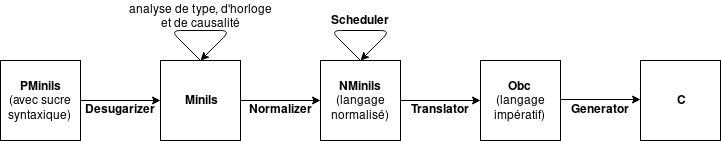
\includegraphics[width=.8\paperwidth]{assets/chain.png}
    Proche de l'organisation décrite dans~\citep{Biernacki08}
  \end{center}
\end{frame}

\section{Polymorphisme d'horloge (et horloges implicites)}

\section{Automates}

\section{Interpréteur et vérification}

\section{AVR-Lustre}

\section{Demo !}

\begin{frame}
  \printbibliography
\end{frame}

\end{document}
